\documentclass[11pt, a4paper, english]{NTNUoving}
\usepackage[utf8]{inputenc}
\usepackage[T1]{fontenc}
\usepackage{float}
\usepackage{enumitem}
\usepackage{csquotes}
\usepackage{algorithm}
\usepackage{algorithmic}
\usepackage{listings}
\usepackage{listings}
\usepackage{color}
\usepackage{biblatex}
\usepackage{hyperref}
\ovingnr{7}    % Nummer på innlevering
\semester{Spring 2021}
\fag{Optimization and Control \\ TTK4135}
\institutt{Department for Engineering Cybernetics}

\definecolor{mygreen}{RGB}{28,172,0} % color values Red, Green, Blue
\definecolor{mylilas}{RGB}{170,55,241}


\begin{document}

\lstset{language=Matlab,%
    %basicstyle=\color{red},
    breaklines=true,%
    morekeywords={matlab2tikz},
    keywordstyle=\color{blue},%
    morekeywords=[2]{1}, keywordstyle=[2]{\color{black}},
    identifierstyle=\color{black},%
    stringstyle=\color{mylilas},
    commentstyle=\color{mygreen},%
    showstringspaces=false,%without this there will be a symbol in the places where there is a space
    numbers=left,%
    numberstyle={\tiny \color{black}},% size of the numbers
    numbersep=9pt, % this defines how far the numbers are from the text
    emph=[1]{for,end,break},emphstyle=[1]\color{red}, %some words to emphasise
    %emph=[2]{word1,word2}, emphstyle=[2]{style},
}

%1
\begin{oppgave}
    Choosing:
    $I = S$, $BR^{-1}B^\top P = UTV$, $R^{-1} = T \implies T^{-1} = R$,
    $VS^{-1}U = B^\top P B \implies U = B \wedge V = B^\top P$.
    These were chosen to match it with the expected result (6).
    By the matrix inversion lemme this gives us:
    \begin{align*}
        (I + BR^{-1}B^\top P)^{-1} &= I - IB(R + B^\top PIB)^{-1} B^\top PI
    \end{align*}
    Inserting this into (5) gives us:
    \begin{align*}
        P &= Q + A^\top P(I - IB(R + B^\top PIB)^{-1} B^\top PI)A \\
        &= Q + A^\top P A - A^\top P B (R + B^\top PB)^{-1})B^\top PA \\
        0 &= Q + A^\top P A - A^\top P B (R + B^\top PB)^{-1})B^\top PA - P
    \end{align*}
    Which is (6).
\end{oppgave}

\begin{oppgave}
    \begin{punkt}
    The code used is shown below.
    \lstinputlisting{../task2a.m}
    Results in $K = \begin{bmatrix}
        1.0373 \\
        1.6498
    \end{bmatrix}$
    and $e = \text{eig}(A - BK) = 0.8675 \pm 0.0531i$
    \end{punkt}

    \begin{punkt}
        The code used is shown below, I used the poles suggested by the task.
        \lstinputlisting{../task2b.m}

        This resulted in the graph shown in Figure \ref{fig:2b}.

        \begin{figure}[H]
            \centering
            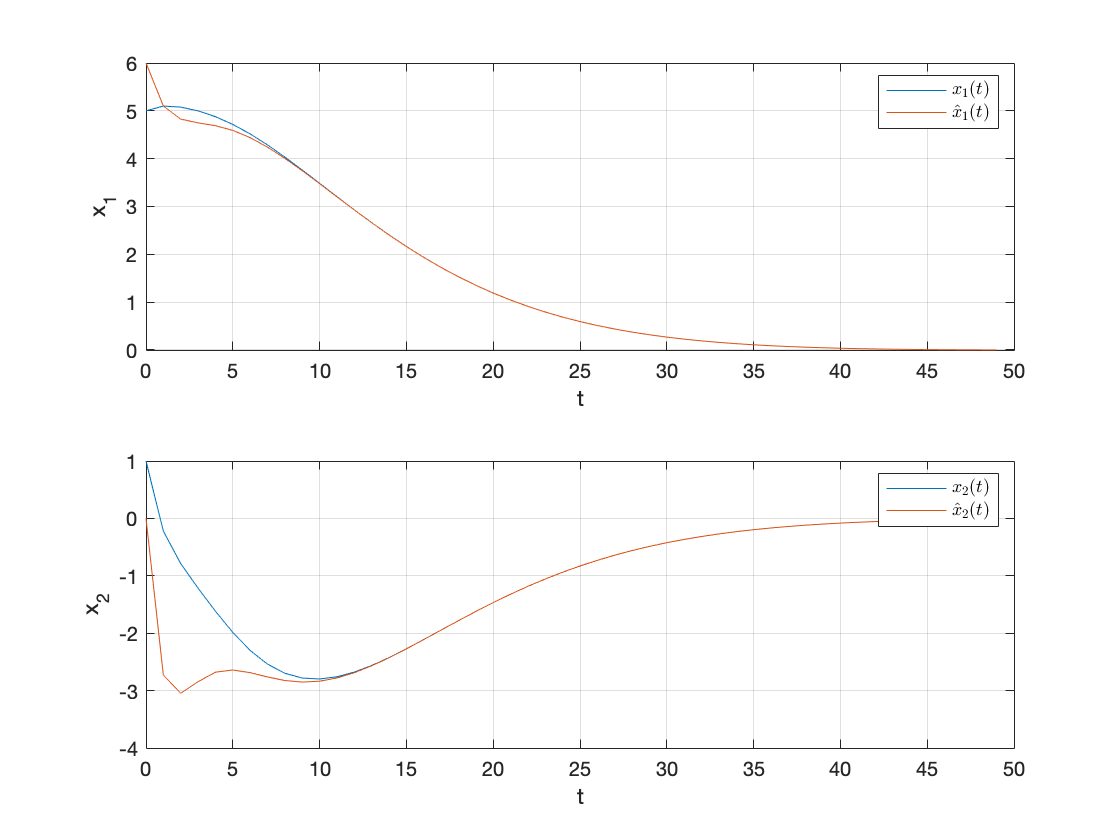
\includegraphics[width=1.0\textwidth]{../task2b.png}
            \caption{LQR with output feedback.}
            \label{fig:2b}
        \end{figure}
        As we can see the estimated state converges pretty quickly towards the real state. The controller
        uses some time to converge towards the origin, but manages to do it within 50 time steps.
    \end{punkt}

    \begin{punkt}
        We have that:
        \begin{align*}
            BK &= \begin{bmatrix}
                0 \\ 0.1
            \end{bmatrix} \begin{bmatrix}
                1.0373 & 1.6498
            \end{bmatrix} = \begin{bmatrix}
                0 & 0 \\
                0.10373 & 0.16498
            \end{bmatrix} \\
            A - BK &= \begin{bmatrix}
                1 & 0.1 \\
                -0.1 & 0.9
            \end{bmatrix} - \begin{bmatrix}
                0 & 0 \\
                0.10373 & 0.16498
            \end{bmatrix} = \begin{bmatrix}
                1 & 0.1 \\
                -0.2037 & 0.7350
            \end{bmatrix} \\
            A - K_F C &= \begin{bmatrix}
                1 & 0.1 \\
                -0.1 & 0.9
            \end{bmatrix} - \begin{bmatrix}
                0.9 \\ 1.509
            \end{bmatrix} \begin{bmatrix}
                1 & 0
            \end{bmatrix}
            = \begin{bmatrix}
                0.1 & 0.1 \\
                -1.609 & 0.9
            \end{bmatrix}
            \\
        \implies \Phi &= \begin{bmatrix}
            1 & 0.1 & 0 & 0 \\
            -0.2037 & 0.7350 & 0.10373 & 0.16498 \\
            0 & 0 & 0.1 & 0.1 \\
            0 & 0 & -1.609 & 0.9
        \end{bmatrix}
        \end{align*}
        Using \texttt{eig} in Matlab to find the eigen values of $\Phi$:
        \begin{align*}
            \lambda_1 &= 0.8675 \pm 0.0530i \\
            \lambda_2 &= 0.5 \pm 0.03i
        \end{align*}
        Which are the poles we got earlier.
    \end{punkt}
\end{oppgave}

\begin{oppgave}
    \begin{punkt}

        The code used is shown below.
        \lstinputlisting{../task3a.m}

        The results are given in Figure \ref{fig:3a}.
        \begin{figure}[H]
            \centering
            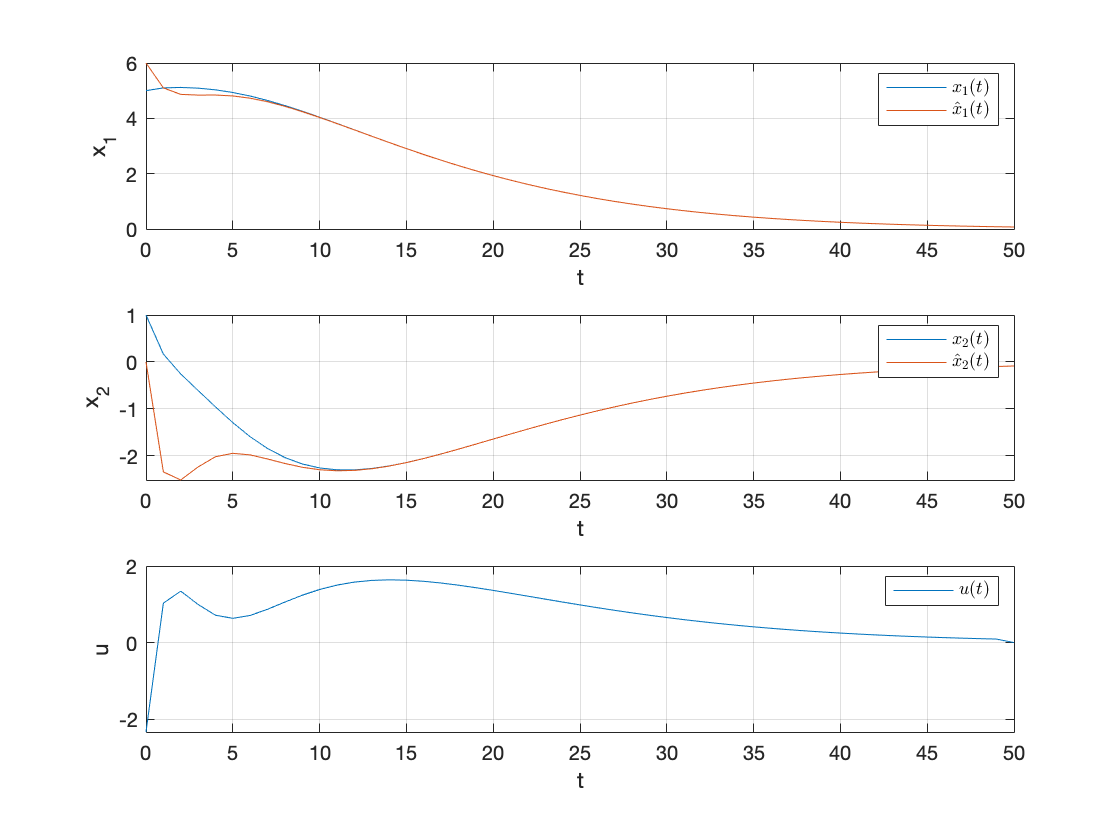
\includegraphics[width=1.0\textwidth]{../task3a.png}
            \caption{MPC with output feedback.}
            \label{fig:3a}
        \end{figure}
    \end{punkt}

    The code used is shown below.
    \lstinputlisting{../task3a.m}

    \begin{punkt}

        The results are given in Figure \ref{fig:3b}.
        \begin{figure}[H]
            \centering
            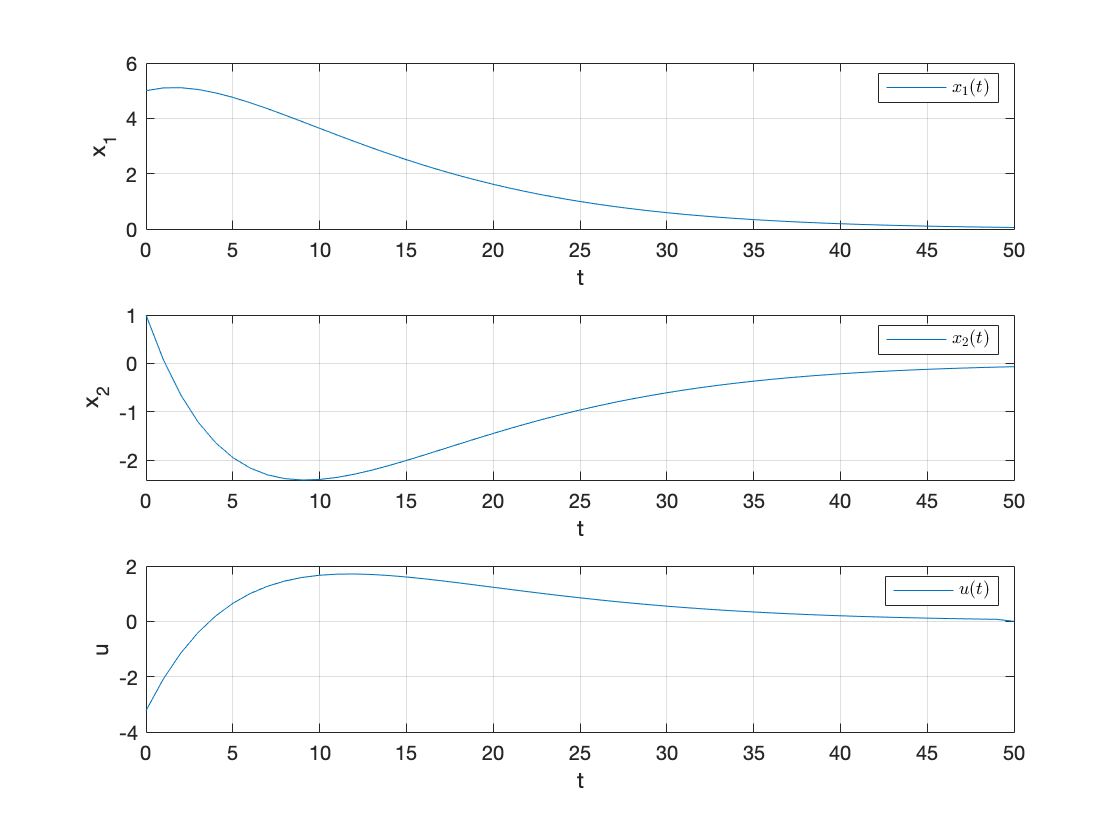
\includegraphics[width=1.0\textwidth]{../task3b.png}
            \caption{MPC with state feedback.}
            \label{fig:3b}
        \end{figure}
    \end{punkt}
\end{oppgave}

\begin{oppgave}
    \begin{punkt}

        $P$ was gotten in Problem 1:
        \begin{align*}
            P &= \begin{bmatrix}
                27.5170  &  7.2713 \\
                7.2713  & 10.2339
            \end{bmatrix}
        \end{align*}
    \end{punkt}

    \begin{punkt}
        The code used is shown below.
    \lstinputlisting{../task4b.m}

    The results are given in Figure \ref{fig:4b}.
    \begin{figure}[H]
        \centering
        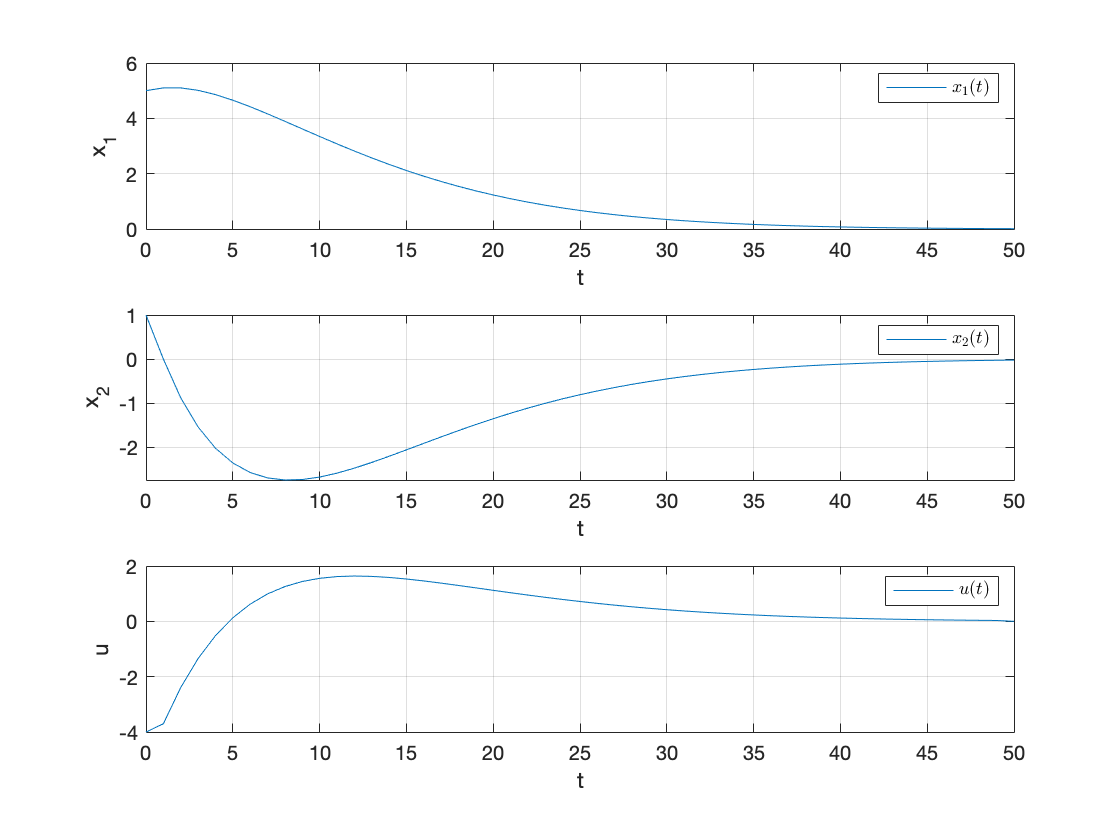
\includegraphics[width=1.0\textwidth]{../task4b.png}
        \caption{MPC with state feedback and infinite horizon.}
        \label{fig:3b}
    \end{figure}
    We can see that this MPC converges slightly faster towards the origin than the MPC from Problem 3b.
    Changing $N$ did not change the solution much, as far as my testing went (from values 1-30), the control input constraints
    where inactive except for the first few control inputs. $N$ becomes more important for performance in realistic scenarios
    without state feedback and when there are clearer performance goals, like runtime or memory constraints.
    \end{punkt}
\end{oppgave}

\end{document}
